\chapter{网络应用}
为检验FPGA加速网络协议的效果,我们基于ClickNP平台开发了五个常见的网络应用。

\section{包生成器(PktGen)及抓包器(PktCap)}
包生成器可根据不同的配置生成不同模型、不同大小的网络包,通过流量控制器,以不同的速率和猝发程度发出。

抓包器将收到的包记录为日志存储在主机上。由于记录单个日志元件无法充分利用PCIe通信带宽,
抓包器通过在FPGA内建的接收端扩放元件将收到的包根据头部散列值分散到多个日志元件中。
鉴于PCIe通道带宽低于网络的40Gbps,我们在记录包的时候只提取我们最感兴趣的16字节字段,
与4字节的时间戳一起经PCIe通道发送至主机上的日志元件。

抓包器的设计体现了CPU与FPGA协同工作的重要性。相比于FPGA而言,CPU有更大的存储空间,
且更容易访问固态硬盘等其他存储器,因而将日志元件部署在CPU上有利于提升性能。

\section{OpenFlow防火墙(OFW)}
我们的OpenFlow\cite{McKeown:2008:OEI:1355734.1355746}防火墙支持对网络流量进行精确匹配及模糊匹配两种工作方式。
精确匹配表通过布谷鸟散列算法\cite{Pagh2001}实现,支持128K条包头记录。
模糊匹配基于三态结合存储器(ternary content-addressable memory, TCAM)实现,
然而实现三态结合存储器的完整功能在FPGA上开销过大\cite{Bosshart:2013:FMF:2486001.2486011},
一个包含512条记录的TCAM就会占用芯片上超过50\%的资源。
因此我们在实现中取而代之采用散列三态结合存储器(hashed ternary content-addressable memory, HASH-TCAM)实现。
HASH-TCAM将表空间分解为一系列更小的散列表,每个散列表对应一个掩码位,所有输入的包在散列之前都先经过一次按位与操作。
散列表中每条记录都被赋予优先级,通过仲裁逻辑选出优先级最高的记录,如图~\ref{fig:hashtcam} 所示。
\begin{figure}[htbp]
\centering
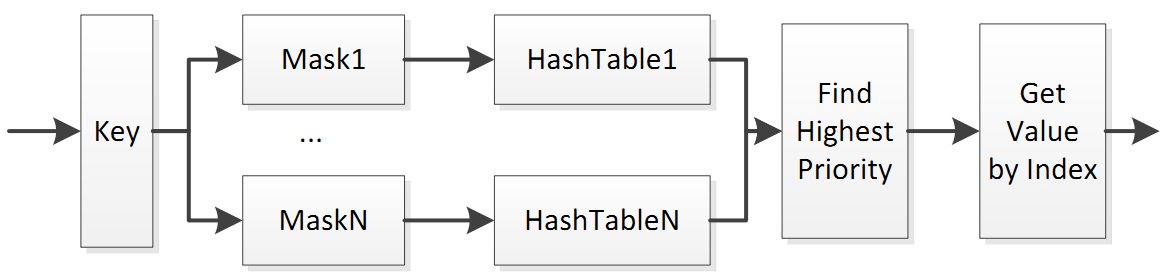
\includegraphics[width=4in]{hashtcam}
\caption{散列三态结合存储器实现模糊匹配规则} \label{fig:hashtcam}
\end{figure}

散列三态结合存储器通过在容量方面的让步,节省了大量空间开销。
在我们的实现中,HASH-TCAM采用16个不同的掩码位,支持16K条流记录。

\section{互联网安全协议网关(IPSecGW)}
软件网络功能面临的一个困难是在IPSec等计算密集型系统中CPU成为性能瓶颈\cite{Han:2010:PGS:1851275.1851207}。
我们搭建了一条互联网安全协议数据通路,可以对IPSec包进行AES-256-CTR加密以及SHA-1认证。

因为一个AES\_CTR元件能达到的最大带宽为27.8Gbps,而链路带宽为40Gbps,
于是我们让两个AES\_CTR元件并行地工作,以充分利用带宽。

对于SHA-1认证而言,数据被分为64字节的小块。虽然对于单个数据块的计算可以流水化,
但同一个互联网协议包的相邻数据块之间存在数据依赖,即后一个块的计算需要等待前一个块计算完成才可以开始。
倘若将这些数据块串行处理,其吞吐率低达1.07Gbps。

我们的解决方法是在不同的包之间进行数据级并行:在后一级流水处理一个包的数据块时,
前一级流水处理另一个包的数据块。这样消除了两个数据块之间的数据依赖,
使其可以并行处理。

为了实现这一设计,我们设计了暂存元件,可以缓冲多达64个包并向SHA-1元件调度彼此独立的数据块。在计算完一个包的签名后,
暂存元件将其发送至下一级元件来生成散列运算消息认证码(hash-based message authentication code, HMAC)并将其追加至包末尾。

\section{第4层负载均衡(L4LB)}
我们仿照Ananta\cite{Patel:2013:ACS:2486001.2486026}中的数据选择器实现了第4层负载均衡。总体而言,
该数据选择器检查包头部来判断该流是否有分配直接地址(direct address, DIP)。
如果有,则该包将通过IP in IP隧道转发至直接地址指定的服务器;
否则,数据选择器将调用本地控制器为该流分配一个直接地址。
我们在ClickNP中实现了这一功能,将除了分配直接地址(DIPAlloc)以外的其他元件部署在FPGA上。
这是因为每个流只有第一个包才可能触发分配直接地址元件,且分配的计算过程教复杂,
部署在FPGA上一方面造成计算资源紧张,另一方面可能拖慢时钟频率。

面对流量极大的数据中心网络,第四层负载均衡需要记录多达3200万个流。
如此大的流表显然超出块存储器和FPGA的存储能力,
需要存放在板载双倍速率随机存储器(double data rate random access memory, DDR RAM)中。
FPGA对DDR SDRAM的访问速度较慢,因此我们在块存储器中搭建了含16K条记录的4路组相连流缓存,
通过最久未使用(least recent used, LRU)算法进行缓存置换。

\section{pFabric流调度器}
pFabric调度器\cite{Alizadeh:2013:PMN:2486001.2486031}工作原理较简单:维护一个包含32个包的缓冲优先队列。最高优先级的包最先出队,
缓冲区满时换出优先级最低的包。pFabric调度可实现数据中心包处理时间的近似最优。

原论文作者提出用二叉查找树组织数据。虽然二叉查找树计算最高优先级的包只需要$log_2N$个时钟周期,
但该过程存在数据依赖,致使为了使吞吐率达到链路带宽上限40Gbps,时钟频率需要高达300MHz,
这对于现有的FPGA平台而言是不可能的。

我们采取了另一种更容易并行化的实现方式:通过移位寄存器实现优先队列\cite{895938},
包以优先级降序记录在K个寄存器中,如图~\ref{fig:pfabric} 所示。
每次出队操作将所有记录右移,弹出队首,仅消耗1个时钟周期。
对于入队操作,新包的元数据被转发给所有记录。每条记录将新包与自身及左右邻居的优先级进行比较,
优先级最低的记录经本地比较后自行被换出。因为所有的本地比较操作可以并行执行,所以入队操作也仅消耗1个时钟周期。
入队与出队操作也能够实现并行化,因而每个包都只需要1个时钟周期即可处理完成。
\begin{figure}[htbp]
\centering
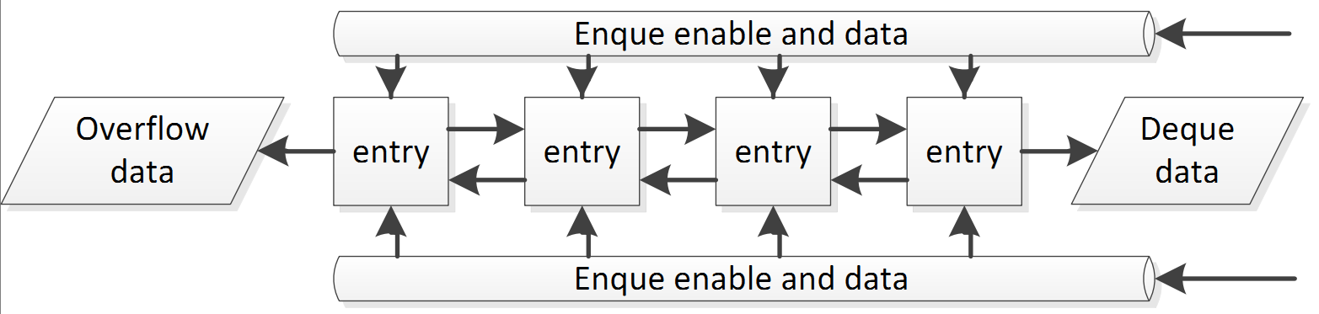
\includegraphics[width=4in]{pfabric}
\caption{移位寄存器实现pFabric流调度} \label{fig:pfabric}
\end{figure}
